\chapter{Исследовательский раздел}
\label{cha:research}

Тестирование программы проводилось на 2.7 GHz 2‑ядерном процессоре Intel Core i5 с встроенной видеокартой
Intel Iris Graphics 6100 на 1536 МБ и на 3.59 GHz 8-ядерном процессоре AMD Ryzen 7 3700x с дискретной
видеокартой NVidia GeForce RTX 2060 на 6144 МБ. В обоих случаях использовалось разрешение 1920 на 1080
точек.

\section{Исследование характеристик программы}

На рисунке \ref{img:plot} видна зависимость кадров в секунду от количества частиц.
В данном тесте проводилась визуализация облаков, каждое из которых состояло из 14400 частиц.

\begin{figure}[H]
    \begin{tikzpicture}
        \begin{axis}[
            legend pos = north east,
            xlabel=Количество частиц,
            ylabel=Кадры в секунду,
            grid = major,
            width = 0.8\paperwidth,
            height = 0.38\paperheight,
            line width = 1
        ]

            \legend{
                Встроенная видеокарта,
                Дискретная видеокарта
            };

            \addplot[color=black, mark=square] coordinates {
                    (0, 60)
                    (14400, 20)
                    (28800, 12)
                    (43200, 7)
                    (57600, 6)
                    (72000, 5)
                    (86400, 4)
                    (100800, 3)
                    (115200, 3)
                    (129600, 3)
                    (144000, 2)
            };

        \addplot[color=gray, mark=*] coordinates {
                    (0, 60)
                    (14400, 60)
                    (28800, 47)
                    (43200, 32)
                    (57600, 24)
                    (72000, 19)
                    (86400, 16)
                    (100800, 13)
                    (115200, 11)
                    (129600, 10)
                    (144000, 9)
            };
        \end{axis}
    \end{tikzpicture}
    \caption{Количество кадров в секунду в зависимости от количества частиц}
    \label{img:plot}
\end{figure}

\section{Примеры использования программы}

Пример работы программы при добавленном облаке видно на рисунке \ref{img:example1}.

\begin{figure}[H]
    \centering
    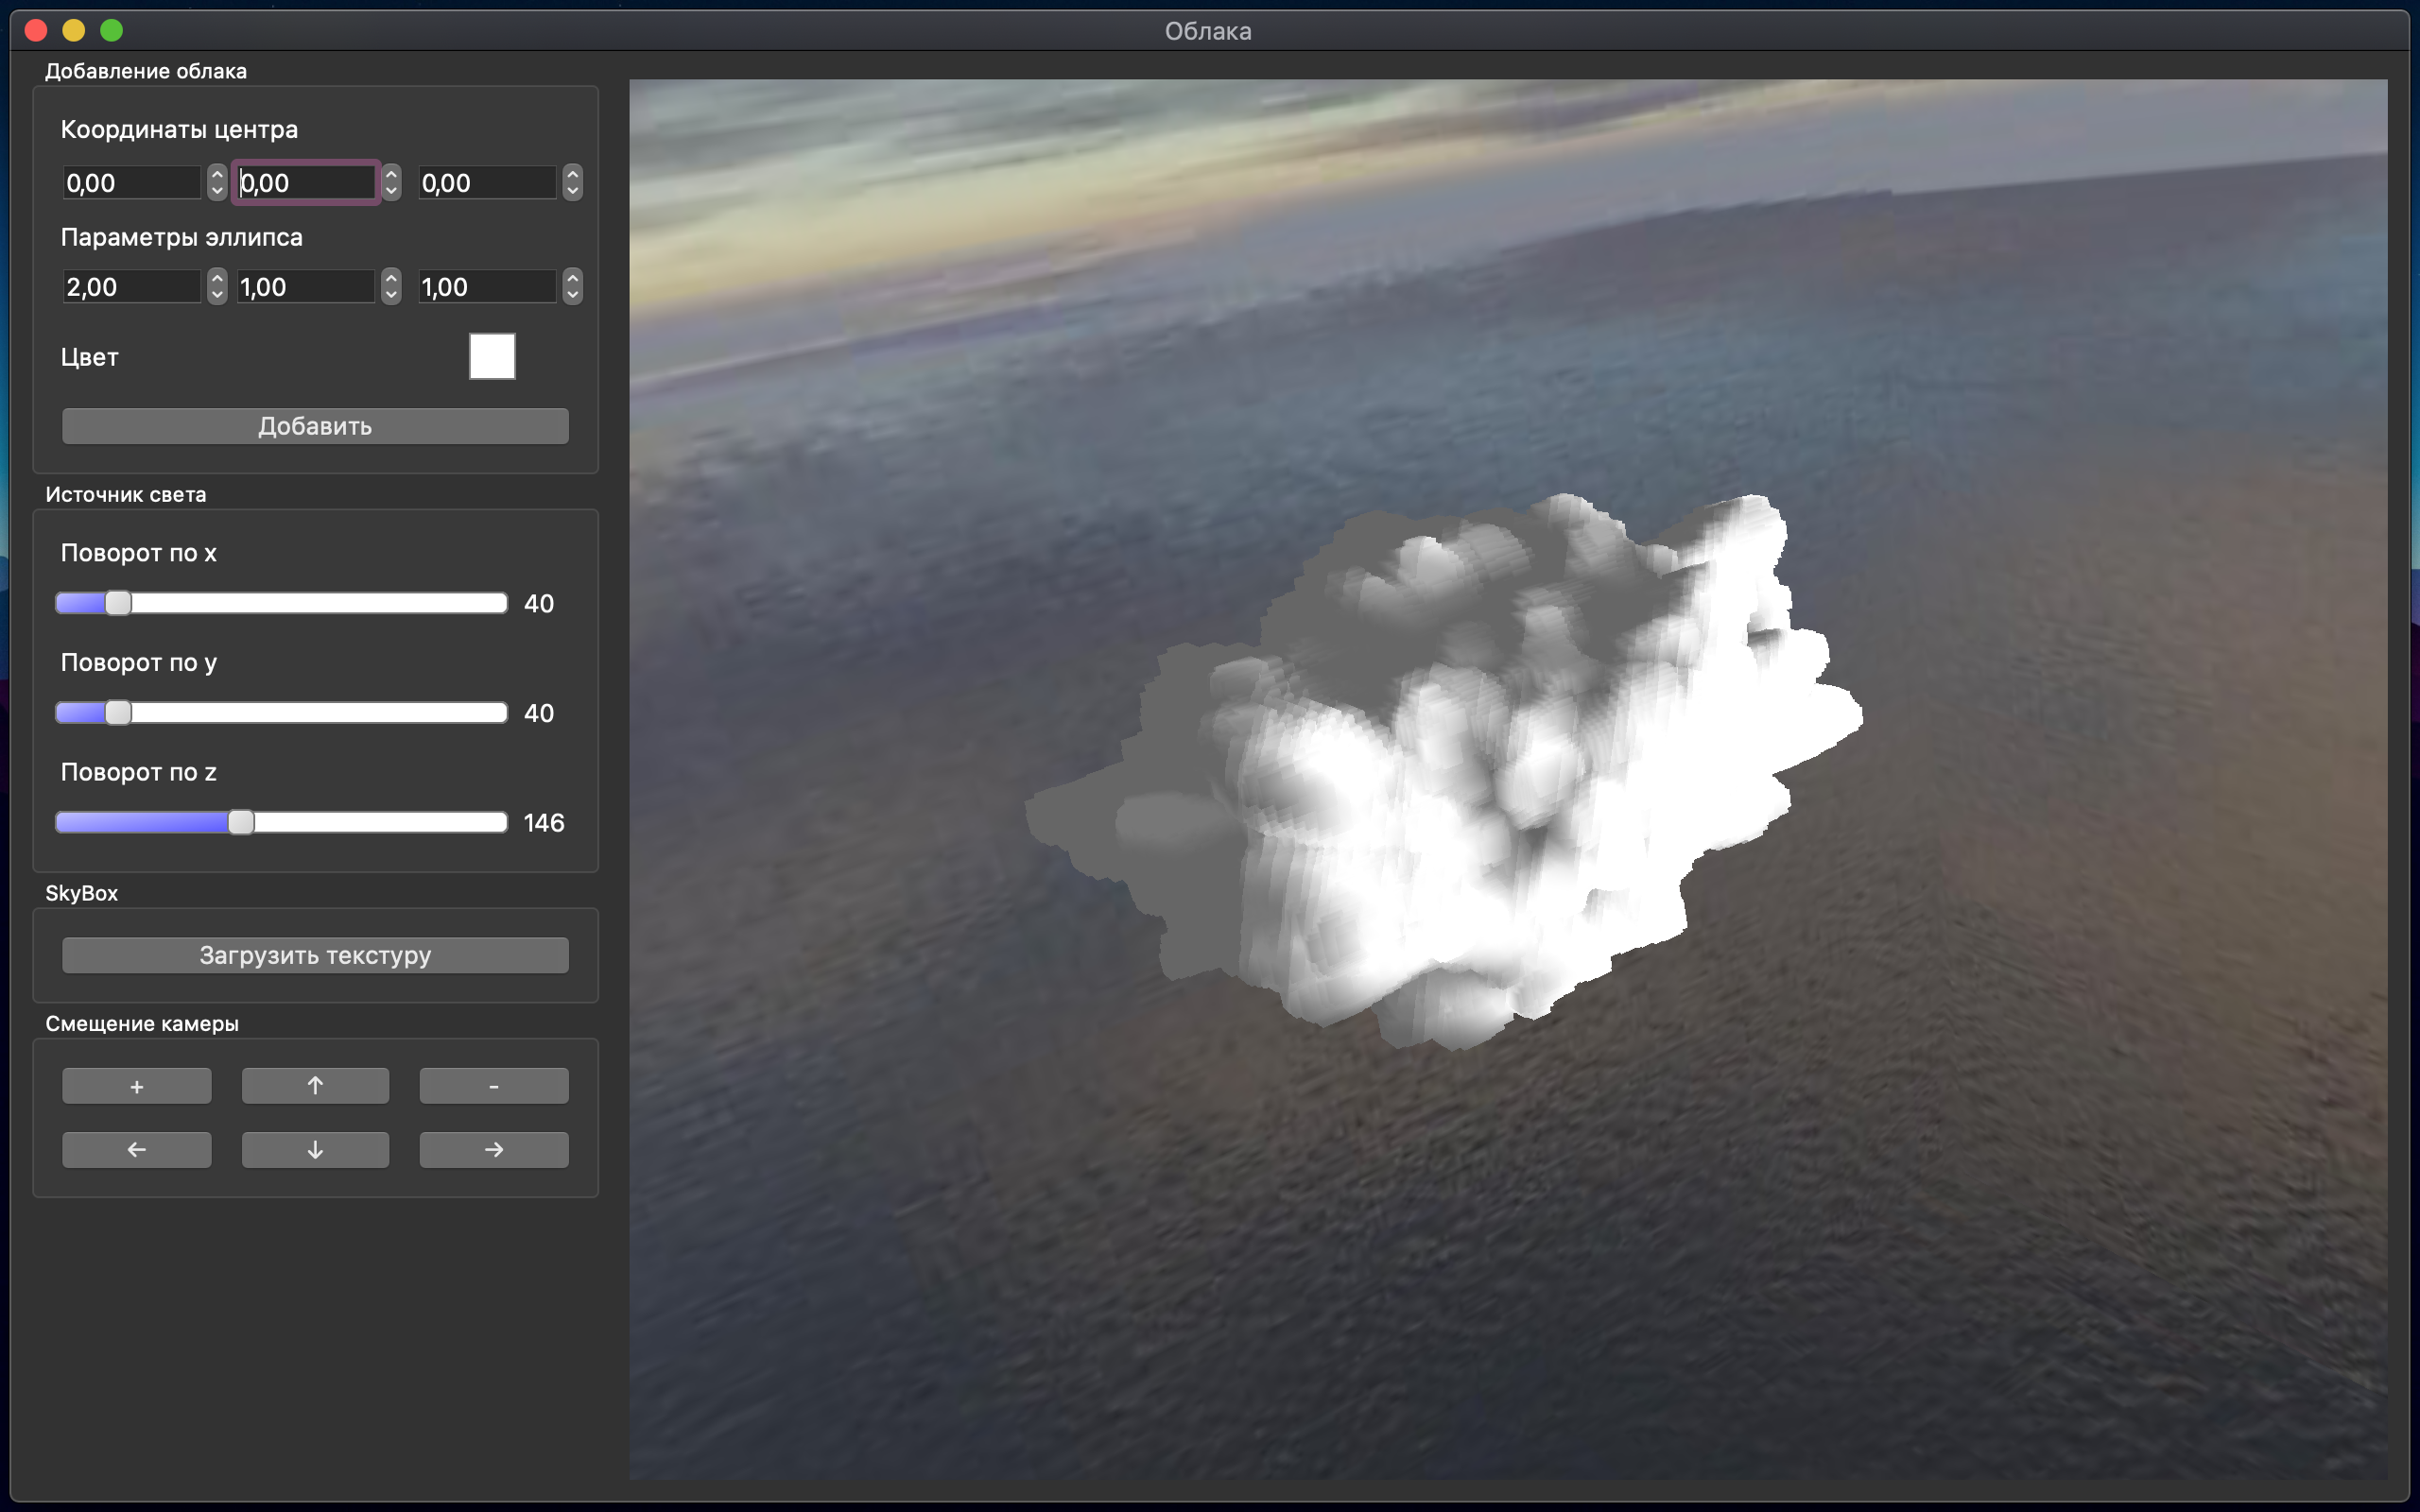
\includegraphics[scale=0.3]{img/example1.png}
    \caption{Пример добавленного облака}
    \label{img:example1}
\end{figure}

После добавления можно использовать камеру, чтобы рассмотреть облако с разных сторон и изменить положение
источника света (рисунок \ref{img:example2}).

\begin{figure}[H]
    \centering
    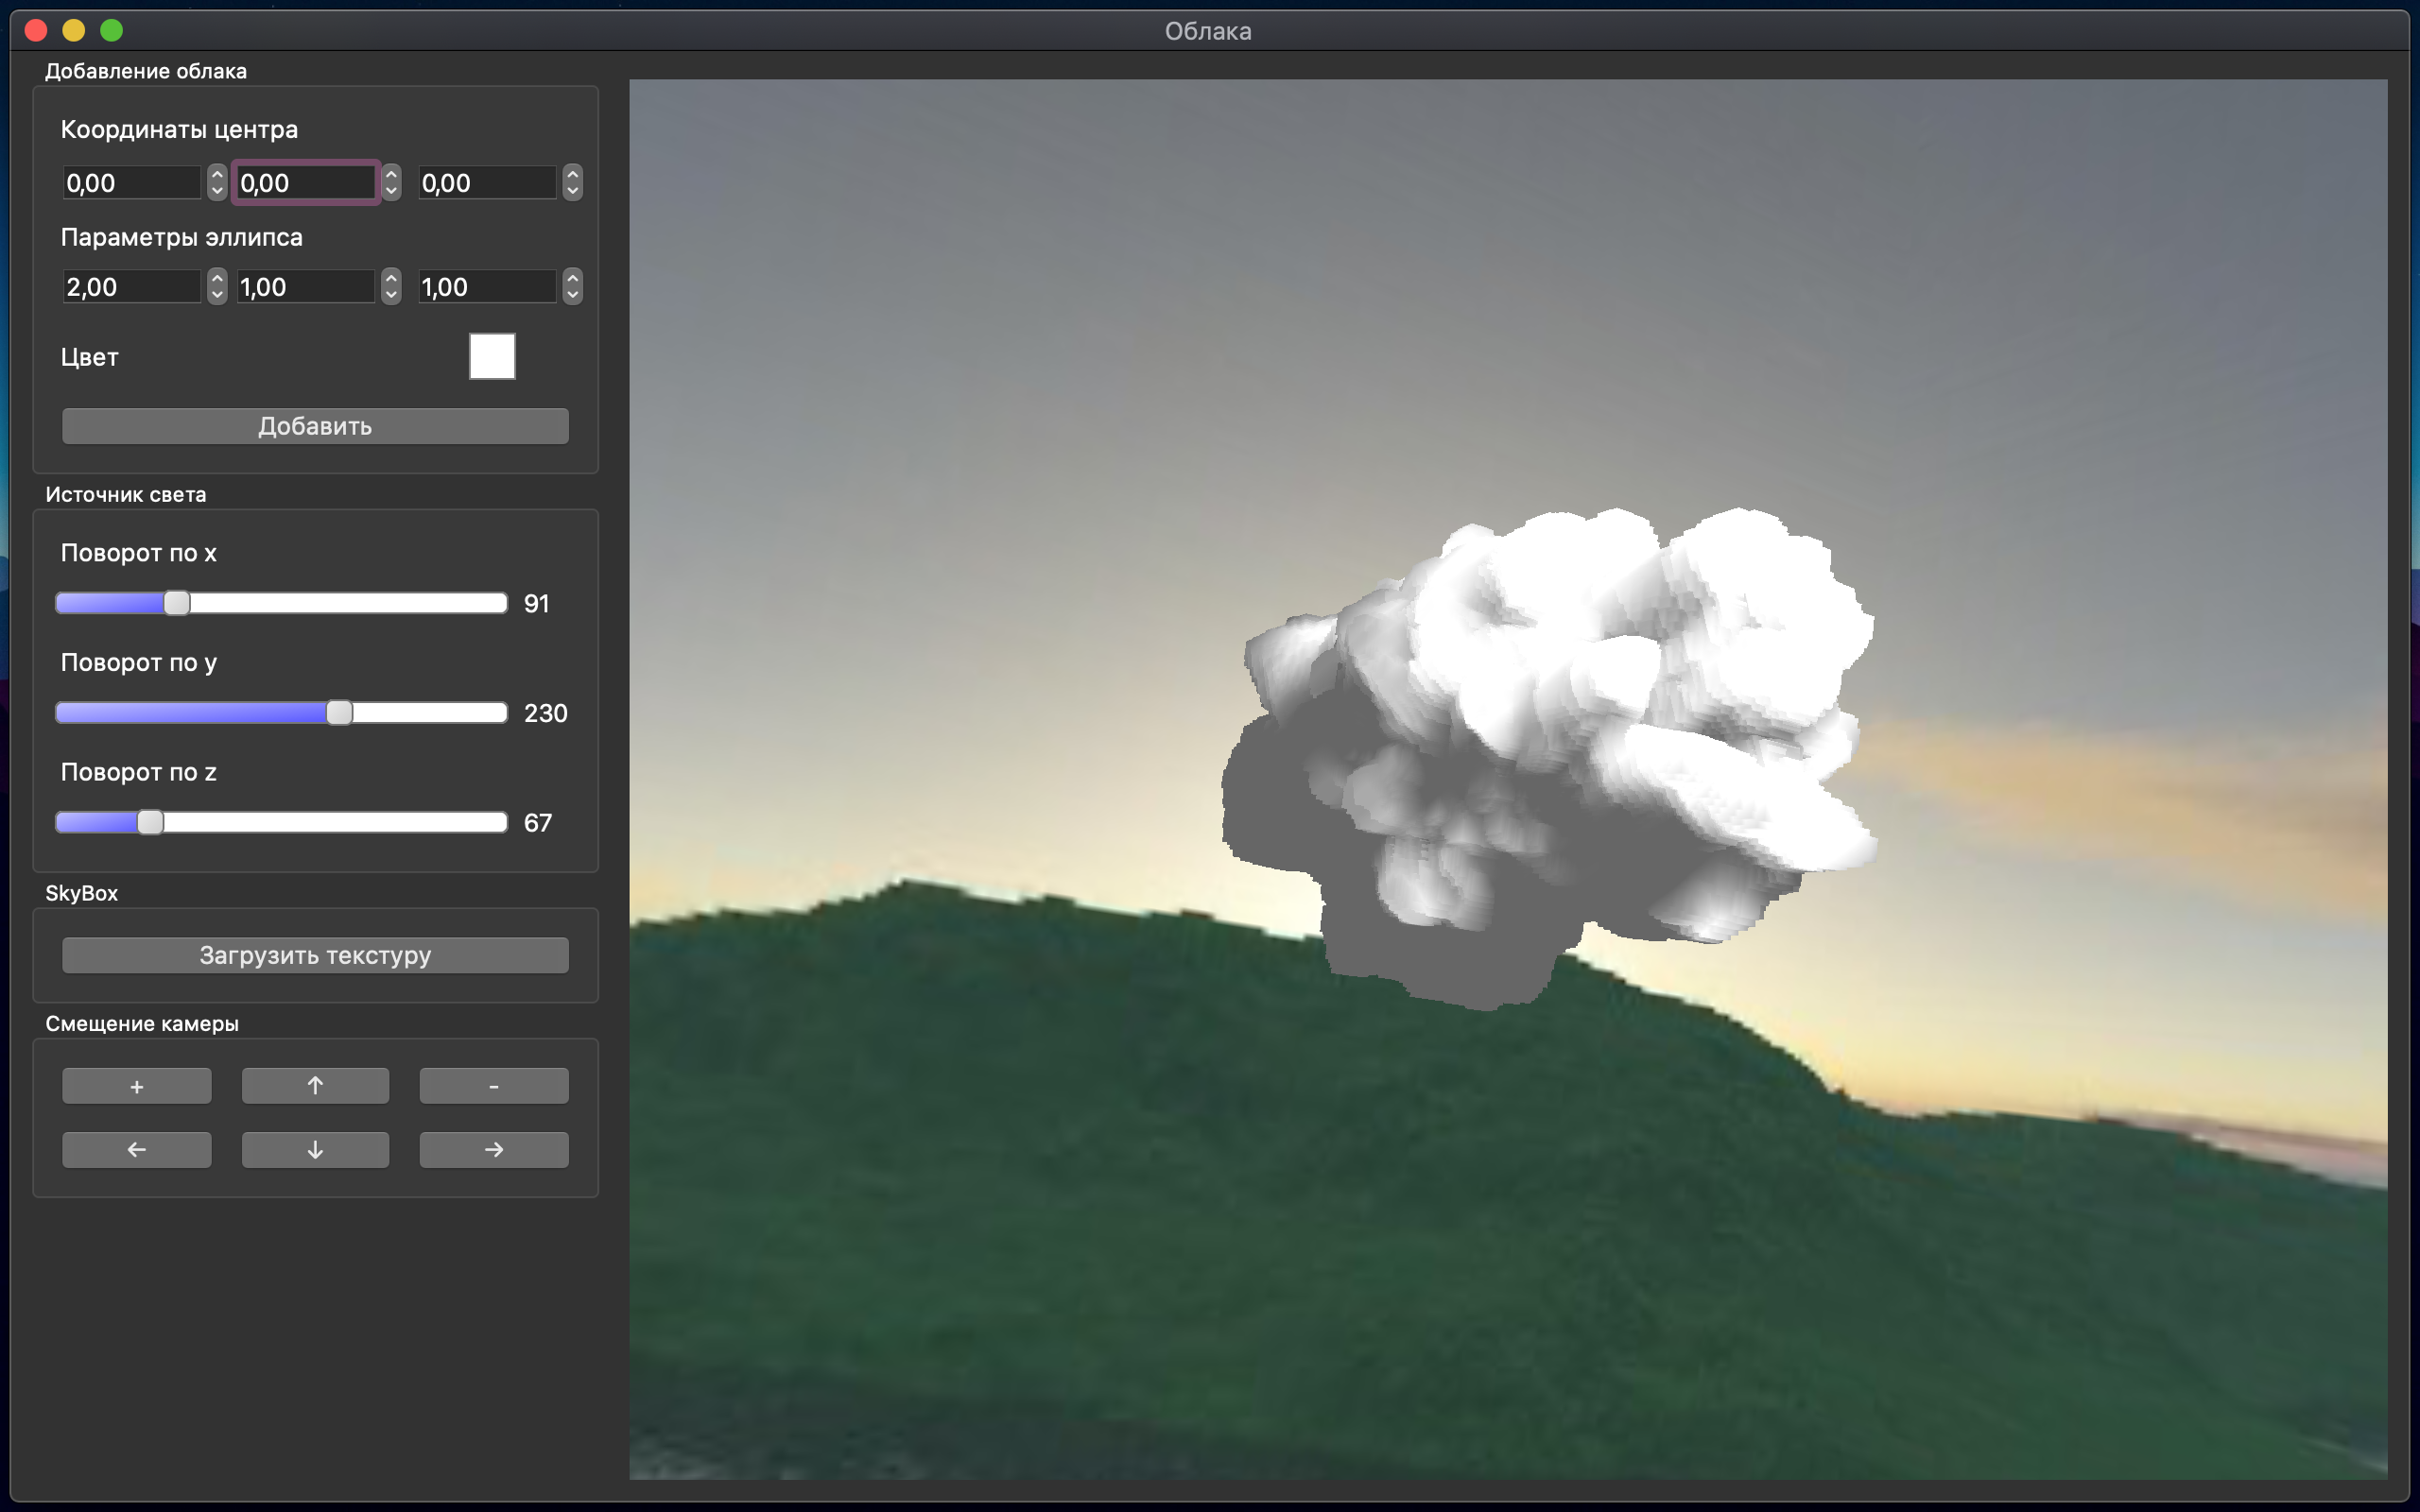
\includegraphics[scale=0.3]{img/example2.png}
    \caption{Пример работы камеры}
    \label{img:example2}
\end{figure}

Также можно поменять текстуру небесного куба, что видно на рисунке \ref{img:example3}.

\begin{figure}[H]
    \centering
    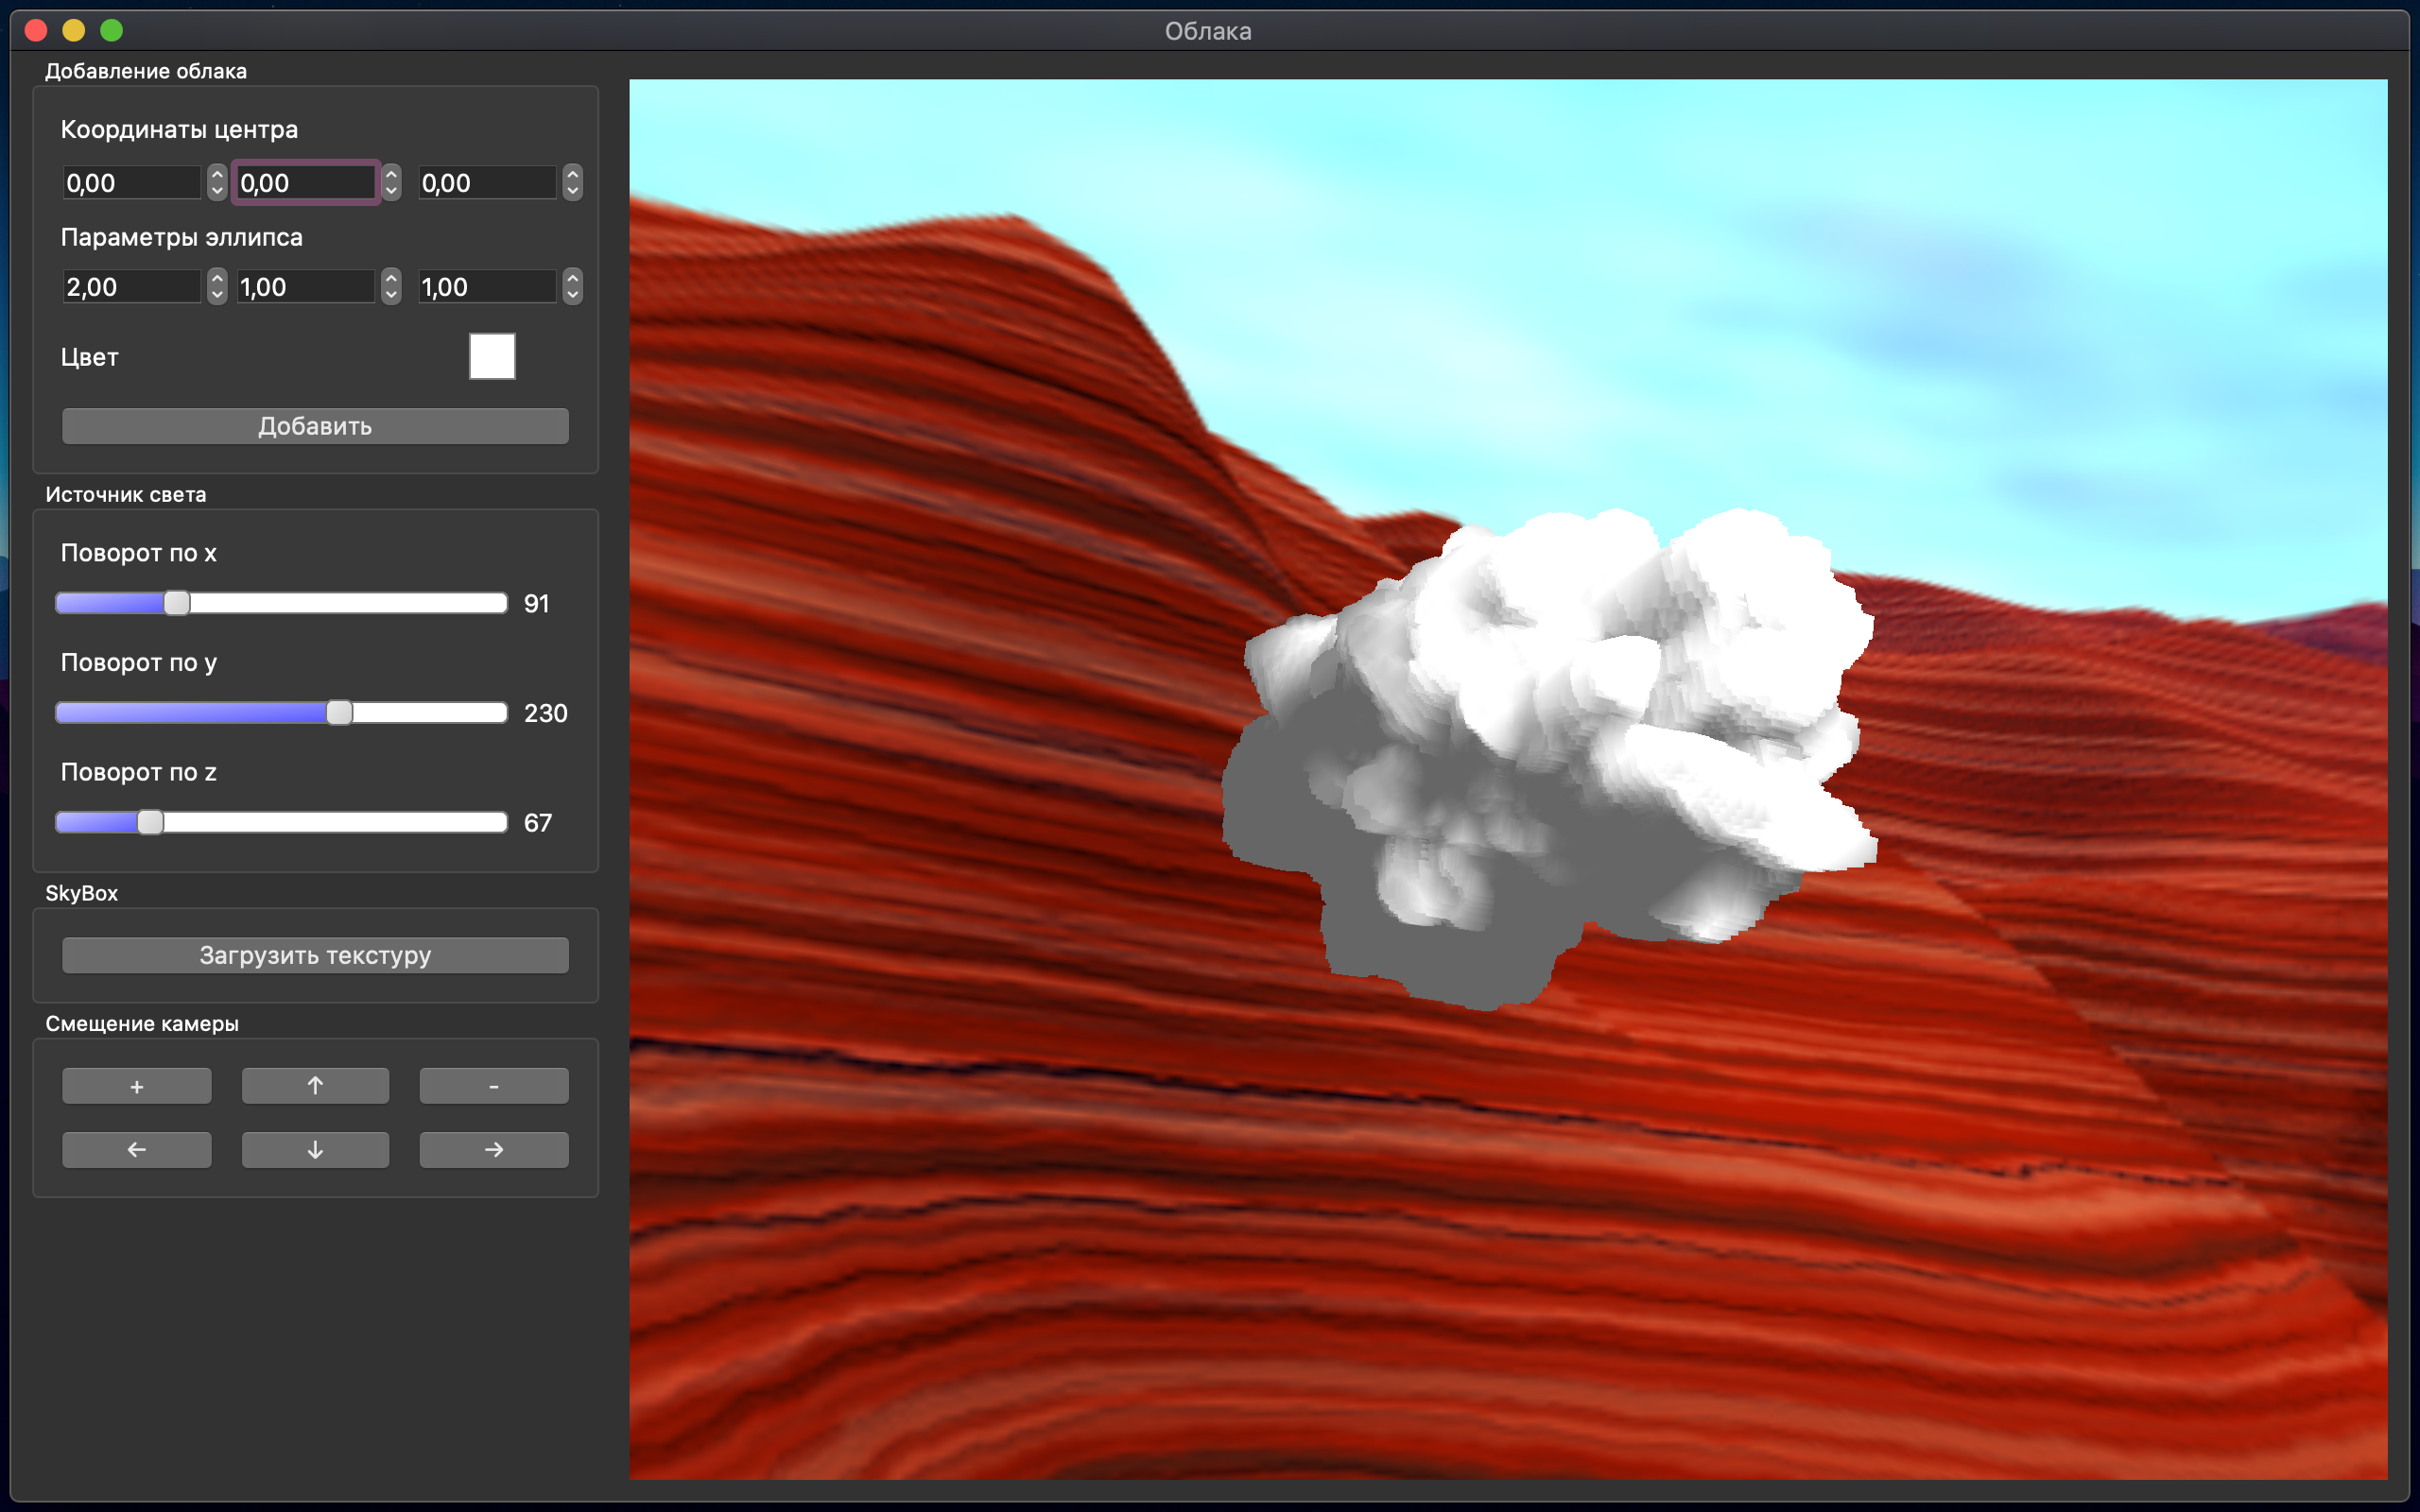
\includegraphics[scale=0.3]{img/example3.png}
    \caption{Пример смены небесного куба}
    \label{img:example3}
\end{figure}

\section{Выводы}

Если используется мощная дискретная видеокарта, то можно использовать до 50000 частиц, получая
частоту кадров больше 30. На встроенной видеокарте получился результат до 10000 частиц.
